\documentclass[final,t]{beamer}

% themes
\usetheme{tb2}

% lang
\usepackage[utf8x]{inputenc} \usepackage[english]{babel}

% others
\usepackage{xspace} \usepackage{hyperref} \usepackage{fancyvrb}
\usepackage{listings}
\lstset{language=python, breaklines=true, belowskip=.5em, aboveskip=.5em}

\usepackage[nolist]{acronym}

\usepackage{enumitem} \setitemize{label=\usebeamerfont*{itemize item}%
  \usebeamercolor[fg]{itemize item} \usebeamertemplate{itemize item}}

% graphics
\usepackage{tikz} \usetikzlibrary{arrows} \usetikzlibrary{backgrounds}
\pgfdeclarelayer{background} \pgfdeclarelayer{foreground}
\pgfsetlayers{background,main,foreground}

\graphicspath{{img/}}


% beamer poster !
\usepackage[orientation=portrait,size=a0,scale=2]{beamerposter}

% extra macros
\newcommand{\email}[1]{\texttt{#1}}

% TODO : Inclure logos
% used to set the footer
\newcommand\beamerposterfooter{%
  \foreach \x in {}{%
    \hfill\includegraphics[height=1.5em]{\x}\hfill%
  }%
}

% Correct a bug in the vertical spacing by added a 'g' phantom,
% because putting some \strut{} at every line was to much to fit on
% the page...
\title{Pythran: automatic python to c++ conversion of scientific
  programs}
    

\author{\normalsize P.~Brunet \and S.~Guelton \and A.~Raynaud}

\institute{\normalsize \vspace{4ex} Telecom Bretagne, Brest }

\begin{document}

\begin{frame}[fragile]
  
  \begin{columns}
    % 
    \column{.03\textwidth}{}
    
    \column{.45\textwidth}{
      \Large
      \begin{itemize}
      \item A python to C++ compiler for a subset of the
        python language.
      \item Makes numerical algorithms written in python run faster.
      \end{itemize}
    }
    
    \column{.04\textwidth}{}
    
    \column{.45\textwidth}{
      \Large
      \begin{itemize}
      \item Can turn a sequential program into a multithreaded
        one using well-known OpenMP directives.
      \end{itemize}
    }
    
    \column{.03\textwidth}{}
    
  \end{columns}
  
  \vspace{\baselineskip}
      
    \begin{columns}

      \column{0.5\textwidth}{

        \vspace{\baselineskip}

        \begin{block}{\Large Pythran compilation}

        \vspace{0.4\baselineskip}
        \large
          \begin{itemize}
            \item Python modules are annotated with some interface description.
            \item Pythran converts them into C++.
            \item After compilation, the native modules are faster
              than the original written in python.
          \end{itemize}
  
        \end{block}

        \begin{block}{\Large Parallelization}

          \vspace{0.4\baselineskip}
          \large 
          \begin{itemize}
            \item OpenMP-like annotations are added to the python modules. 
            \item Pythran converts the annotations into C++ OpenMP directives.
            \item The resulting native modules use multithreading.
          \end{itemize}
  
        \end{block}
      }

      \column{0.5\textwidth}{   

        \vspace{0.4\baselineskip}

        \begin{center}
          \textbf{\Large\color{tbgreen}{Example}}
          \begin{lstlisting}[language=Python]
  #pythran export pi_estimate(int)
  def pi_estimate(DARTS):
    hits = 0
    "omp parallel for private(i,x,y,dist), reduction(+:hits)"
    for i in xrange (0, DARTS):
      x = random()
      y = random()
      dist = sqrt(pow(x, 2) + pow(y, 2))
      if dist <= 1.0:
        hits += 1.0
    pi = 4 * (hits / DARTS)
    return pi
          \end{lstlisting}
        \end{center}
      }

    \end{columns}

  \begin{block}{\Large Results}

    \vspace{\baselineskip}

    \begin{columns}
      
      \column{0.45\textwidth}{
        \vspace{0.4\baselineskip}
        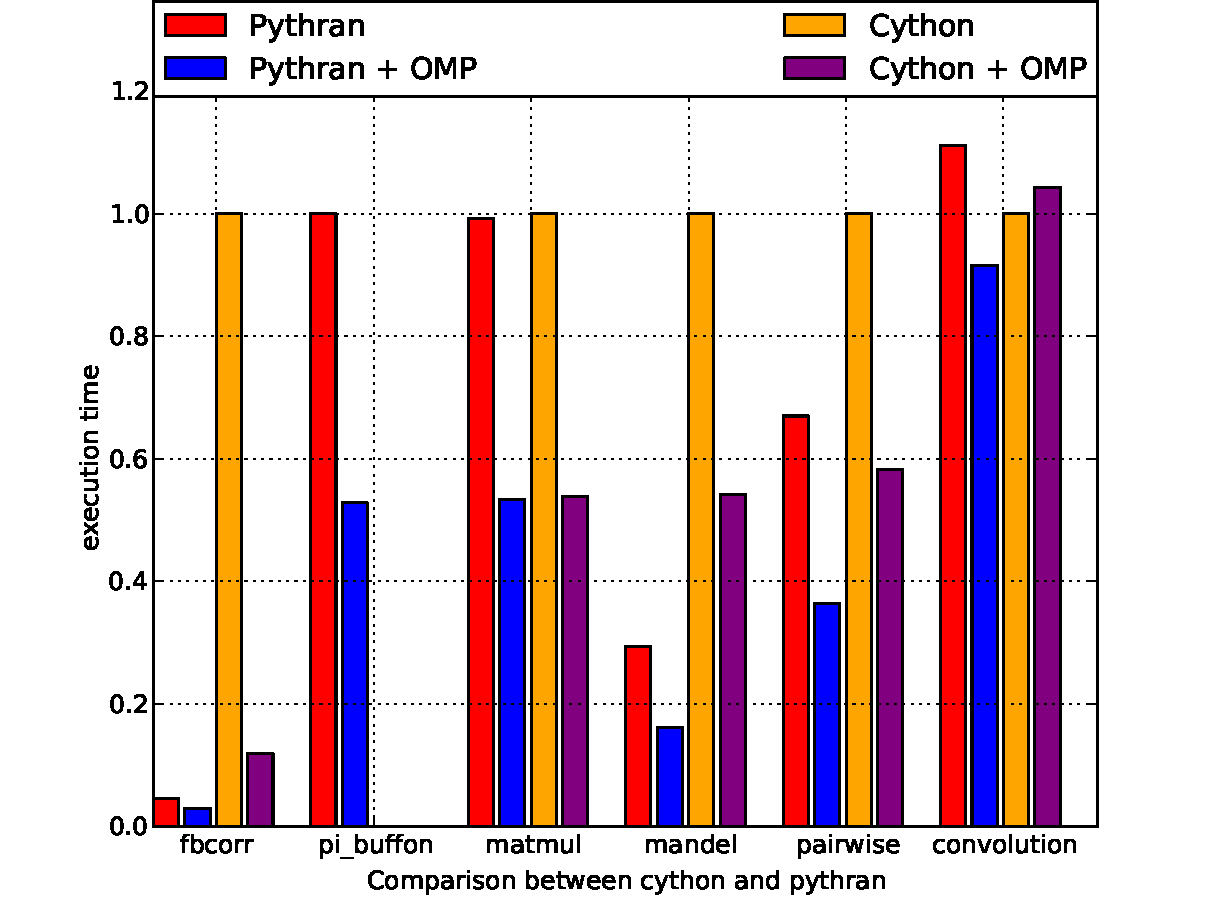
\includegraphics[width=\textwidth]{cython}
      }

      \column{0.55\textwidth}{ 
        \vspace{0.4\baselineskip}

        \begin{itemize}
        \item \large Pythran is far more performant than CPython, the
          standard implementation of Python.
          \begin{itemize}
            \normalsize
          \item Up to 2000x faster.
          \item An additional boost when using parallelism.
          \end{itemize}
        \vspace{0.4\baselineskip}
        \item \large Pythran also compares well with other python
          optimization tools, like PyPy or Cython.
          
        \end{itemize}

      }

    \end{columns}

  \end{block}
  
  
\end{frame}

\end{document}

%%% Local Variables:
%%% mode: latex
%%% mode: tex-pdf
%%% mode: flyspell
%%% ispell-local-dictionary: "american"
%%% End:
